\documentclass{standalone}
\usepackage{pgfplots}
\usepgfplotslibrary{statistics, groupplots}
\pgfplotsset{compat=1.18}

\begin{document}
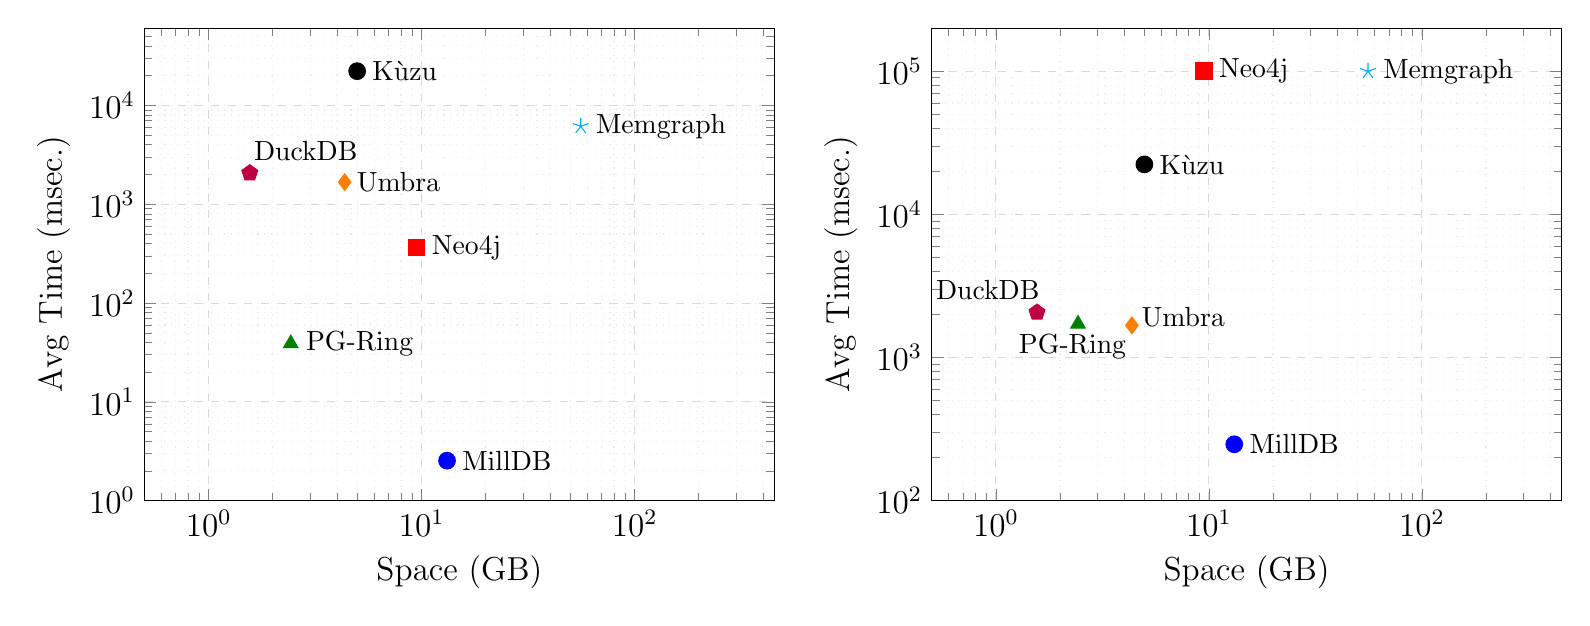
\begin{tikzpicture}[font=\large]
    \begin{groupplot}[
            group style={
                group size=2 by 1,
                horizontal sep=2cm,
            },
            height=6cm,
            width=8cm,
            scale only axis,
            grid=both,                          % Activa rejilla mayor y menor
            grid style={dashed, gray!30},       % Estilo rejilla principal
            minor grid style={dotted, gray!15}, % Estilo rejilla pequeña (más tenue)
            minor y tick num=9,                 % 9 marcas entre potencias de 10
        ]

    % --- PRIMER GRÁFICO (SCATTER) ---
    \nextgroupplot[
        xlabel={Space (GB)},
        ylabel={Avg Time (msec.)},
        xmin = 0.5, ymode = log,
        ymin = 1, xmode = log,
        scatter/classes={
            a={mark=*,blue}, b={mark=square*,red}, c={mark=triangle*,green!50!black},
            d={mark=diamond*,orange}, e={mark=pentagon*,purple}, f={mark=otimes*,black}, g={mark=star,cyan}
        },
        enlarge x limits={abs=70pt, upper},
    ]
    \addplot[scatter, only marks, scatter src=explicit symbolic, mark size=3pt]
    table[x=x, y=y, meta=class] {
        x   y       class
        13.16  2.54     a
        9.47  364.14     b
        2.43  38.94     c
        4.35  1674.44     d
        1.56  2069.88    e
        4.98  22215.51   f
        55.85 6172.53    g
    };

    \node[anchor=west, font=\normalsize, xshift=2pt] at (axis cs:13.16,2.54) {MillDB};
    \node[anchor=west, font=\normalsize, xshift=2pt] at (axis cs:9.47,364.14) {Neo4j};
    \node[anchor=west, font=\normalsize, xshift=2pt] at (axis cs:2.43,38.94) {PG-Ring};
    \node[anchor=east, font=\normalsize, xshift=38pt] at (axis cs:4.35,1674.44) {Umbra};
    \node[anchor=west, font=\normalsize, xshift=-2pt, yshift=8pt] at (axis cs:1.56,2069.88) {DuckDB};
    \node[anchor=west, font=\normalsize, xshift=2pt] at (axis cs:4.98,22215.51) {Kùzu};
    \node[anchor=west, font=\normalsize, xshift=2pt] at (axis cs:55.85,6172.53) {Memgraph};

    % --- SEGUNDO GRÁFICO (SCATTER) ---
        \nextgroupplot[
            xlabel={Space (GB)},
            ylabel={Avg Time (msec.)},
            xmin = 0.5, ymode = log,
            ymin = 100, xmode = log,
            scatter/classes={
                        a={mark=*,blue}, b={mark=square*,red}, c={mark=triangle*,green!50!black},
                        d={mark=diamond*,orange}, e={mark=pentagon*,purple}, f={mark=otimes*,black}, g={mark=star,cyan}
                    },
            enlarge x limits={abs=70pt, upper},
        ]
        \addplot[scatter, only marks, scatter src=explicit symbolic, mark size=3pt]
        table[x=x, y=y, meta=class] {
            x   y       class
            13.16  247.70     a
            9.47   100030.90     b
            2.43  1716.22     c
            4.35  1677.02     d
            1.56  2066.58    e
            4.98  22338.35   f
            55.85 100045.75    g
        };

        \node[anchor=west, font=\normalsize, xshift=2pt] at (axis cs:13.16,247.70) {MillDB};
        \node[anchor=west, font=\normalsize, xshift=2pt] at (axis cs:9.47,100030.90) {Neo4j};
        \node[anchor=south, font=\normalsize, xshift=-2pt, yshift=-16pt] at (axis cs:2.43,1716.22) {PG-Ring};
        \node[anchor=west, font=\normalsize, yshift=3pt] at (axis cs:4.35,1677.02) {Umbra};
        \node[anchor=west, font=\normalsize, xshift=-40pt, yshift=8pt] at (axis cs:1.56,2066.58) {DuckDB};
        \node[anchor=west, font=\normalsize, xshift=2pt] at (axis cs:4.98,22338.35) {Kùzu};
        \node[anchor=west, font=\normalsize, xshift=2pt] at (axis cs:55.85,100045.75) {Memgraph};




    \end{groupplot}
\end{tikzpicture}
\end{document}